\documentclass[t]{beamer}

% Load general definitions
% Preamble file - general definitions, package loading, etc.

%=================================
% Load packages
\usepackage{amssymb,amsmath}
\usepackage{graphicx}
\usepackage{url}
\usepackage{tikz}
\usetikzlibrary{mindmap,trees,arrows}
\usepackage{fancyvrb}
\usepackage[english]{babel}
\usepackage[latin1]{inputenc}
\usepackage{subfigure}
\usepackage{times}
\usepackage[T1]{fontenc}
\usepackage{cancel}
\usepackage{color}
\usepackage{listings}

%=================================
% Set mode
\mode<presentation>
{
	\usetheme{Madrid}
	\usecolortheme{whale}
	\useoutertheme{infolines}
	\setbeamercovered{invisible}
}

% Get rid of nav bar
\beamertemplatenavigationsymbolsempty

% Insert frame number at bottom of the page.
\usefoottemplate{\hfil\tiny{\color{black!90}\insertframenumber}} 

%=================================
% Define new commands

\newcommand\Real{{\mathbb{R}}}
%\newcommand{\vi}{\vspace{0.6\baselineskip}}
%\newcommand{\goodgap}{\hspace{\subfigtopskip}\hspace{\subfigbottomskip}}


% Equation environments
\newcommand{\beq}{\begin{equation}}
\newcommand{\eq}{\end{equation}}
\newcommand{\beqs}{\begin{equation*}}
\newcommand{\eqs}{\end{equation*}}
\newcommand{\beqn}{\begin{eqnarray}}
\newcommand{\eqn}{\end{eqnarray}}

% Bold variables
\newcommand{\mbf}[1]{\ensuremath{\mathbf{#1}}}

% Itemization
\newcommand{\bitem}{\begin{itemize}}
\newcommand{\eitem}{\end{itemize}}
\newcommand{\spitem}{\vskip 1em\item}
\newcommand{\bitems}{\begin{itemize}\item}
\newcommand{\benums}{\begin{enumerate}\item}
\newcommand{\eenum}{\end{enumerate}}

% color blocks
\newenvironment{colorblock}[2]{%
\setbeamercolor{block title}{#2}
\begin{block}{#1}}{\end{block}}

% Vertical spacing
\newcommand{\vone}{\vskip 1em}
\newcommand{\vhalf}{\vskip .5em}

% Frame environments
\newenvironment{ftst}[3][t]{%
\begin{frame}{environment=ftst,#1}
\frametitle{#2}
\framesubtitle{#3}}{\end{frame}}

\newenvironment{ftstf}[2]{
\begin{frame}[fragile,environment=ftstf]
\frametitle{#1}
\framesubtitle{#2}}{\end{frame}}

% colors
\definecolor{MyGray}{rgb}{0.5,0.5,0.5}
\definecolor{MyDBGray}{rgb}{0.1,0.1,0.4}
\definecolor{darkgreen}{rgb}{0,0.4,0}
\definecolor{black}{rgb}{0,0,0}
\def\defn#1{{\color{red} #1}}

% Footnote
\renewcommand{\thefootnote}{\alph{footnote}}

% Relaxed footnotes
\newcommand{\lfr}[1]{\let\thefootnote\relax\footnote{\tiny #1}}

% Verbatim environment - using FANCYVRB package
\DefineVerbatimEnvironment%
{rcode}{Verbatim}
{fontsize=\scriptsize}

% Verbatim environment - using LISTINGS package
%\lstnewenvironment{rcode} {\lstset{	language = R,
%									basicstyle = \scriptsize\ttfamily,
%									showspaces = false,
%									showstringspaces = false,
%									showtabs = false,
%									keywordstyle = \color{black}\bfseries,
%									commentstyle = \color{darkgreen},
%									numbers = none,
%									otherkeywords={	<-,
%													ggplot,
%													geom_boxplot,
%													facet_grid,
%													shapiro.test,
%													fligner.test,
%													glht,
%													with},
%									deletekeywords={data,
%													model,
%													residuals,
%													c,
%													axis,
%													default,
%													labels,
%													qq.text}}}%
%{}


% Specific definitions
\title[]{Design and Analysis of Experiments}
\subtitle[]{06 - Simple Comparisons}
\author[]{Felipe Campelo\\{\footnotesize http://orcslab.cpdee.ufmg.br/}}
\institute{Graduate Program in Electrical Engineering}
\date{\scriptsize Belo Horizonte\\March 2015}

\begin{document}

% cover page
\setbeamertemplate{footline}{}
\begin{frame}
\begin{flushright}

\includegraphics[width=.25\textwidth]{../figs/principal_completa3_ufmg}
\end{flushright}
  \titlepage
  \begin{tikzpicture}[remember picture,overlay]
  \node[anchor=south east,xshift=-5pt,yshift=122pt] at (current page.south east) {\tiny Version 2.11};
  \node[anchor=south west,yshift=0pt] at (current page.south west) {
\includegraphics[width=.15\textwidth]{../figs/by-nc-sa.png}};
  \end{tikzpicture}  
\end{frame}

%=====

% quotation page
  \begin{frame}[b]
		\frametitle{}
\begin{columns}[T]
\column{0.7\textwidth}
\flushright{\small ``\textit{If you get a million dollars for research it\\
will be very helpful, of course;\\
but what can really make a difference are\\
the good ideas, recognizing those questions\\
which are really important,\\
which are yet to be answered. 
}''\\
\vspace{1em}
Suzana Herculano-Houzel\\
1972 --\\
Brazilian neuroscientist\\
}
\column{0.3\textwidth}
\begin{tikzpicture}[remember picture,overlay]
\node[anchor=south east,yshift=26pt,xshift=0pt] at (current page.south east)
{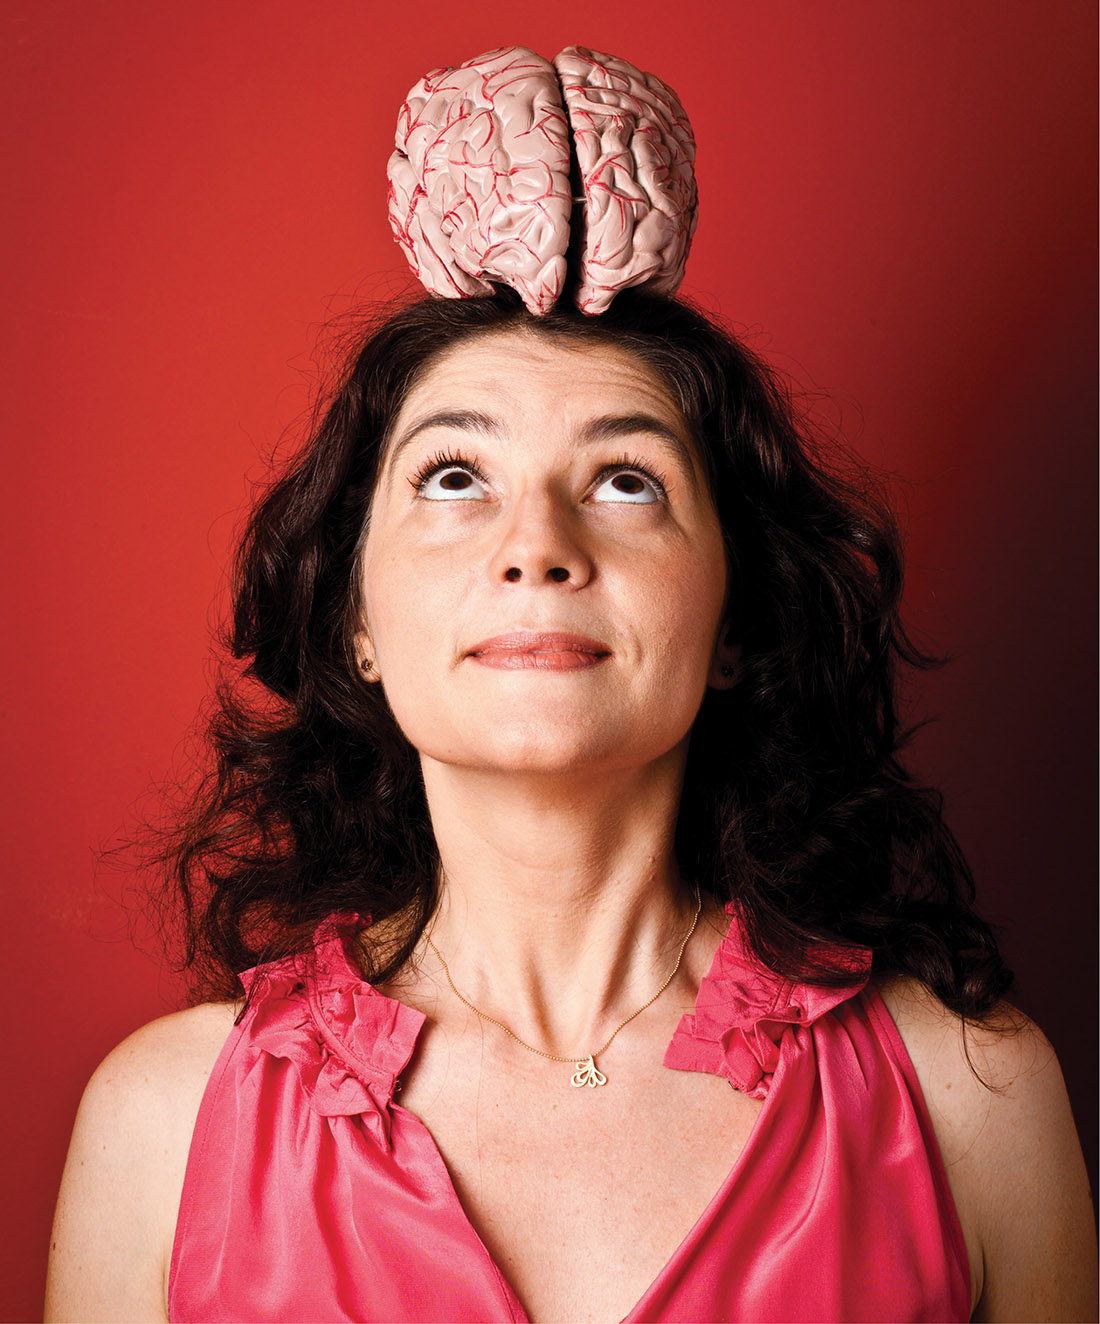
\includegraphics[width=\textwidth]{../figs/SuzanaHouzel.jpeg}};
\end{tikzpicture}
\end{columns}
\vhalf
\lfr{Image by Jorge Bispo: \url{https://goo.gl/KdqQkd}}
\end{frame}

%=====

% Main slides
\begin{ftst}
{Simple Comparative Experiments}
{Statistical inference for two samples}
The concepts of comparison between two populations based on information obtained from their samples follow the same principles used for testing hypotheses about a single population;
\vone
Inferences for two samples frequently arise when comparing the effect of a technique (treatment) against a \textit{control group}: placebo, classical technique, random search, etc;
\vone
Usual questions involve:

\bitems Comparison of means;
\item Comparison of variances;
\item Comparison of proportions;
\item etc.
\eitem
\end{ftst}

%=====

\begin{ftst}
{Comparison of two means}
{Example: Length of steel rods}
\begin{columns}
\column[T]{0.2\textwidth}
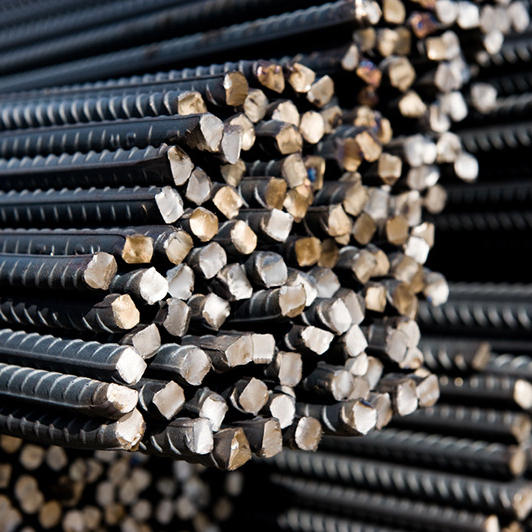
\includegraphics[width=\textwidth]{../figs/steelrods.jpg}
\column[T]{0.8\textwidth}
One of the critical aspects of manufacturing steel rods is cutting the bars with a precise length, which is expected by the customers.
\vhalf
This process is prone to errors, which result in additional costs for standardizing and reprocessing the rods.
\end{columns}
\vone
An engineer is interested in comparing the current controller of the cutting scissors with a new method that could potentially improve the performance of the process.
\lfr{Adapted from D.F. Carvalho Jr.'s course project for the Design and Analysis of Experiments Course, PPGEE-UFMG, June 2012. The data used in this example is not necessarily the original one.}
\lfr{Image: \url{http://www.shutterstock.com/pic-73207399/}}
\end{ftst}

%=====

\begin{ftst}
{Comparison of two means}
{Example: Length of steel rods}
A possible statistical model for this kind of data would be:
\beqs y_{ij} = \mu_i + \epsilon_{ij}\begin{cases}i=1,2\\j=1,\ldots,n_i\end{cases}\eqs
\vone
Lets initially assume that the residuals $\epsilon_{ij}$ are iid $\mathcal{N}\left(0,\sigma_i^2\right)$, which implies:
\lfr{Image: D.C.Montgomery,G.C. Runger, \textit{Applied Statistics and Probability for Engineers},Wiley 2003.}
\begin{tikzpicture}[remember picture,overlay]
\node[anchor=south,yshift=20pt,xshift=0pt] at (current page.south)
{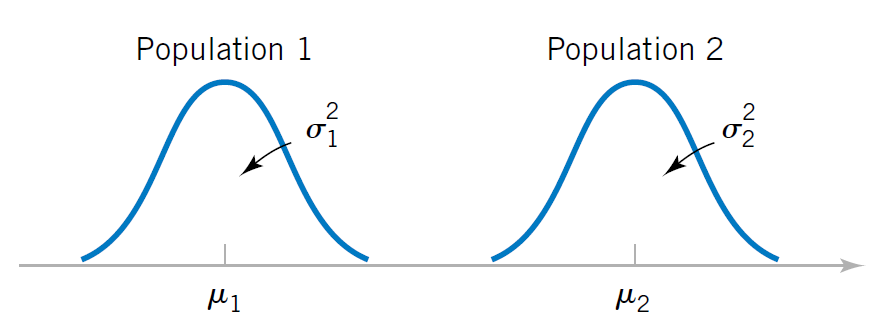
\includegraphics[width=0.8\textwidth]{../figs/popmodels.png}};
\end{tikzpicture}
\end{ftst}

%=====

\begin{ftst}
{Comparison of two means}
{Definitions}
What we wish is to perform an inference about the difference in the mean values of constructive deviations for the two controllers. In this case, a reasonable response variable would be the \textit{absolute error}, from which we could test our hypotheses.
\vhalf
The statistical hypotheses can be stated as:
\beqs
\begin{cases}
H_0: \mu_1 - \mu_2 = 0\\
H_1: \mu_1 - \mu_2 \neq 0
\end{cases}\ \ \ \mbox{\textbf{or, equivalently, }}\ \ \ \ \ \ \begin{cases}
H_0: \mu_1 = \mu_2\\
H_1: \mu_1 \neq \mu_2
\end{cases}
\eqs
\vhalf
Suppose a desired significance level $\alpha = 0.05$, and that the engineer is interested in detecting any difference larger than $15mm$ in the mean absolute error with a power $(1-\beta) = 0.8$.
\vhalf
Also, lets assume that the variance of the process is unknown but similar for both controllers.
\end{ftst}

%=====

\begin{ftst}
{Comparison of two means}
{Definitions}
Since the variance is unknown, it will have to be estimated from the data. As we are assuming $\sigma^2_1\approx\sigma^2_2$, we can use the pooled variance estimator:

\beqs
S_p^2 = \frac{\left(n_1-1\right)S_1^2+\left(n_2-1\right)S_2^2}{n_1+n_2-2}=wS_1^2+\left(1-w\right)S_2^2
\eqs
\vone
Based on this estimator and the stated assumptions, we have that:
\beqs
T = \frac{\left(\bar{y_1} - \bar{y_2}\right) - \left(\mu_1 - \mu_2\right)}{S_p\sqrt{\frac{1}{n_1} + \frac{1}{n_2}}}\sim t_{\left(n_1+n_2-2\right)}
\eqs
\end{ftst}

%=====

\begin{ftst}
{Comparison of two means}
{Rejection threshold}
If we recall our working hypotheses:

\beqs
\begin{cases}
H_0: \mu_1 - \mu_2 = 0\\
H_1: \mu_1 - \mu_2 \neq 0
\end{cases}
\eqs
\vone

\noindent we have that, under $H_0$: 
\beqs 
t_0 = \frac{\left(\bar{y_1} - \bar{y_2}\right) - \cancelto{0}{\left(\mu_1 - \mu_2\right)}}{s_p\sqrt{\frac{1}{n_1} + \frac{1}{n_2}}} = \frac{\left(\bar{y_1} - \bar{y_2}\right)}{s_p\sqrt{\frac{1}{n_1} + \frac{1}{n_2}}}\sim t_{\left(n_1+n_2-2\right)}
\eqs
\vone 
We'll reject $H_0$ at the $(1-\alpha)$ confidence level if $|t_0|\geq t_{1-\alpha/2; (n_1+n_2-2)}$
\end{ftst}

%=====

\begin{ftst}
{Comparison of two means}
{Sample sizes}
Now recall that the process engineer was interested in some very specific characteristics for his test:

\bitems Significance: $\alpha = 0.05$;
\item Power: $(1-\beta) = 0.8$;
\item Minimally interesting effect: $\delta^* = 15mm$
\eitem
\vone
From these specifications, we can obtain the required sample sizes. The derivation of the sample size formulas is not particularly difficult, but we'll concentrate only on the results. More details can be easily found in the literature\footnote[1]{\tiny Check, for instance, Paul Mathews' \textit{Sample Size Calculations}, MMB, 2010.}.
\end{ftst}

%=====

\begin{ftst}
{Comparison of two means}
{Sample sizes}
For the general case of unequal sample sizes, we have:

\beqs
n_1 = \left(1+\frac{n_1}{n_2}\right)\left(\frac{s_p}{\delta^*}\right)^2\left(t_{\alpha/2}+t_{\beta}\right)^2
\eqs
\vhalf

\noindent where $s_p$ is the estimated common standard deviation, and $t_{\alpha/2}$ and $t_{\beta}$ are the $\alpha/2$ and $\beta$ quantiles of the $t_{(n1+n2-2 )}$ distribution. The sample size $n_2$ can be calculated by simply substituting $(n_1/n_2)$ by $(n_2/n_1)$.
\vone
For equal sample sizes $(n_1 = n_2 = n)$ the expression is simplified to:

\beqs
n = 2 \left(\frac{s_p}{\delta^*}\right)^2\left(t_{\alpha/2}+t_{\beta}\right)^2
\eqs
\end{ftst}

%=====

\begin{ftst}
{Comparison of two means}
{Sample sizes}
These formulas are very convenient, but leave us with a riddle: we need variance estimate in order to calculate the sample size, but we need observations to be able to estimate the variance.
\vone
There are a few ways to proceed in this case. The most practical are:
\vhalf
\bitems Use process knowledge or historical data to obtain an (initial) estimate of the  variance;
\spitem Perform a pilot study and collect samples to estimate the variance.
\eitem
\vhalf The first method is almost always preferable since it does not imply additional costs for the experiment.
\end{ftst}

%=====

\begin{ftst}
{Comparison of two means}
{Sample sizes}
If no information is available to estimate the variance, a pilot study must be performed to obtain this value. The sample size required for this pilot study is given by:
\beqs
n_{\mbox{\textit{pilot}}}\approx 2\left(\frac{z_{\alpha_n/2}}{e_{n}}\right)^2
\eqs
\vhalf

\noindent where $(1-\alpha_{n})$ is the desired confidence level for the sample size estimate of the main study, and $e_n$ is the maximum relative error allowed for the sample size.
\vhalf
This calculation can yield some scarily large sample sizes for a pilot study (much larger than would be actually required for the main study itself), so use this with caution.
\end{ftst}

%=====

\begin{ftst}
{Comparison of two means}
{Sample sizes}
For the steel rods experiment, suppose that the engineer uses data available from the controller manuals, as well as historical measurements, to estimate the common standard deviation for the cutting process as $\hat{\sigma} \approxeq 15mm$.
\vhalf
Assuming that equal sample sizes are desired, we can simply use the formula:
\beqs
n = 2 \left(\frac{\hat{\sigma}}{\delta^*}\right)^2\left(t_{\alpha/2}+t_{\beta}\right)^2
\eqs
\vone
Easy, right?
\end{ftst}

%=====

\begin{ftst}
{Comparison of two means}
{Sample sizes}
For the steel rods experiment, suppose that the engineer uses data available from the controller manuals, as well as historical measurements, to estimate the common standard deviation for the cutting process as $\hat{\sigma} \approxeq 15mm$.
\vhalf
Assuming that equal sample sizes are desired, we can simply use the formula:
\beqs
n = 2 \left(\frac{\hat{\sigma}}{\delta^*}\right)^2\left(t_{\alpha/2}+t_{\beta}\right)^2
\eqs
\vone
Easy, right?
\begin{tikzpicture}[remember picture,overlay]
\node[anchor=south east,yshift=0pt,xshift=0pt] at (current page.south east) {
\includegraphics[width=.4\textwidth]{../figs/boromir.jpg}};
\end{tikzpicture}
\end{ftst}

%=====

\begin{ftst}
{Comparison of two means}
{Sample sizes}
The last problem we have to solve is that the values of $t_{\alpha/2}$ and $t_{\beta}$ are also dependent of $n$, which makes the equation
\beqs
n = 2 \left(\frac{\hat{\sigma}}{\delta^*}\right)^2\left(t_{\alpha/2}+t_{\beta}\right)^2
\eqs
\vhalf transcendental in $n$. We'll have to iterate until we find the smallest $n$ that satisfies:
\beqs
n \geq 2 \left(\frac{\hat{\sigma}}{\delta^*}\right)^2\left(t_{\alpha/2}+t_{\beta}\right)^2
\eqs
\vhalf
Usually $t_{\alpha/2}\approx z_{\alpha/2}$ is used for the first iteration. Easy, right?
\end{ftst}

%=====

\begin{ftst}
{Comparison of two means}
{Sample sizes}
The last problem we have to solve is that the values of $t_{\alpha/2}$ and $t_{\beta}$ are also dependent of $n$, which makes the equation
\beqs
n = 2 \left(\frac{\hat{\sigma}}{\delta^*}\right)^2\left(t_{\alpha/2}+t_{\beta}\right)^2
\eqs
\vhalf transcendental in $n$. We'll have to iterate until we find the smallest $n$ that satisfies:
\beqs
n \geq 2 \left(\frac{\hat{\sigma}}{\delta^*}\right)^2\left(t_{\alpha/2}+t_{\beta}\right)^2
\eqs
\vhalf
Usually $t_{\alpha/2}\approx z_{\alpha/2}$ is used for the first iteration. Easy, right?
\lfr{Image: http://vigilantmeadow.deviantart.com/art/DON-T-PANIC-165415311}
\begin{tikzpicture}[remember picture,overlay]
\node[anchor=south east,yshift=-5pt,xshift=0pt] at (current page.south east) {
\includegraphics[width=.15\textwidth]{../figs/dontpanic.png}};
\end{tikzpicture}
\end{ftst}

%=====

\begin{ftstf}
{Comparison of two means}
{Example: Length of steel rods}
Required sample size:
\begin{rcode}
> ss.calc<-power.t.test(delta=15,
                        sd=15,
                        sig.level=0.05,
                        power=0.8,
                        type="two.sample",
                        alternative="two.sided")

Two-sample t test power calculation
n = 16.71477
delta = 15
sd = 15
sig.level = 0.05
power = 0.8
alternative = two.sided

NOTE: n is number in *each* group
\end{rcode}
\end{ftstf}

%=====

\begin{ftstf}
{Comparison of two means}
{Example: Length of steel rods}
Computationally, we can perform the t-test for comparing the means of two independent populations by:
\vhalf
\begin{rcode}
> y<-read.table("../data files/steelrods.txt",
+               header=T)

> with(y,
+      t.test(Length.error~Process, 
+             alternative = "two.sided", 
+             mu = 0, 
+             var.equal = TRUE, 
+             conf.level = 0.95))

Two Sample t-test
data:  Length.error by Process
t = -14.312, df = 32, p-value = 1.849e-15
alternative hypothesis: true difference in means is not equal to 0
95 percent confidence interval:
 -0.09272982 -0.06962312
sample estimates:
mean in group new mean in group old 
       0.07782353        0.15900000 
\end{rcode}
\end{ftstf}

%=====

\begin{ftstf}
{Comparison of two means}
{Example: Length of steel rods}
The assumptions of the test must be verified. In this particular case:

\bitems \alert{Normality of the residuals};
\item Equality of variance of the residuals;
\item Independence of the residuals.
\eitem
\begin{rcode}
> resid<-y$Length.error - rep(means[2:1],
+                             each=n)

> shapiro.test(resid)
Shapiro-Wilk normality test
data:  resid
W = 0.9552, p-value = 0.176

> library(car)
> qqPlot(resid,
+        pch=16,
+        cex=1.5,
+        las=1)
\end{rcode}
\begin{tikzpicture}[remember picture,overlay]
\node[anchor=south east,yshift=-10pt,xshift=10pt] at (current page.south east) {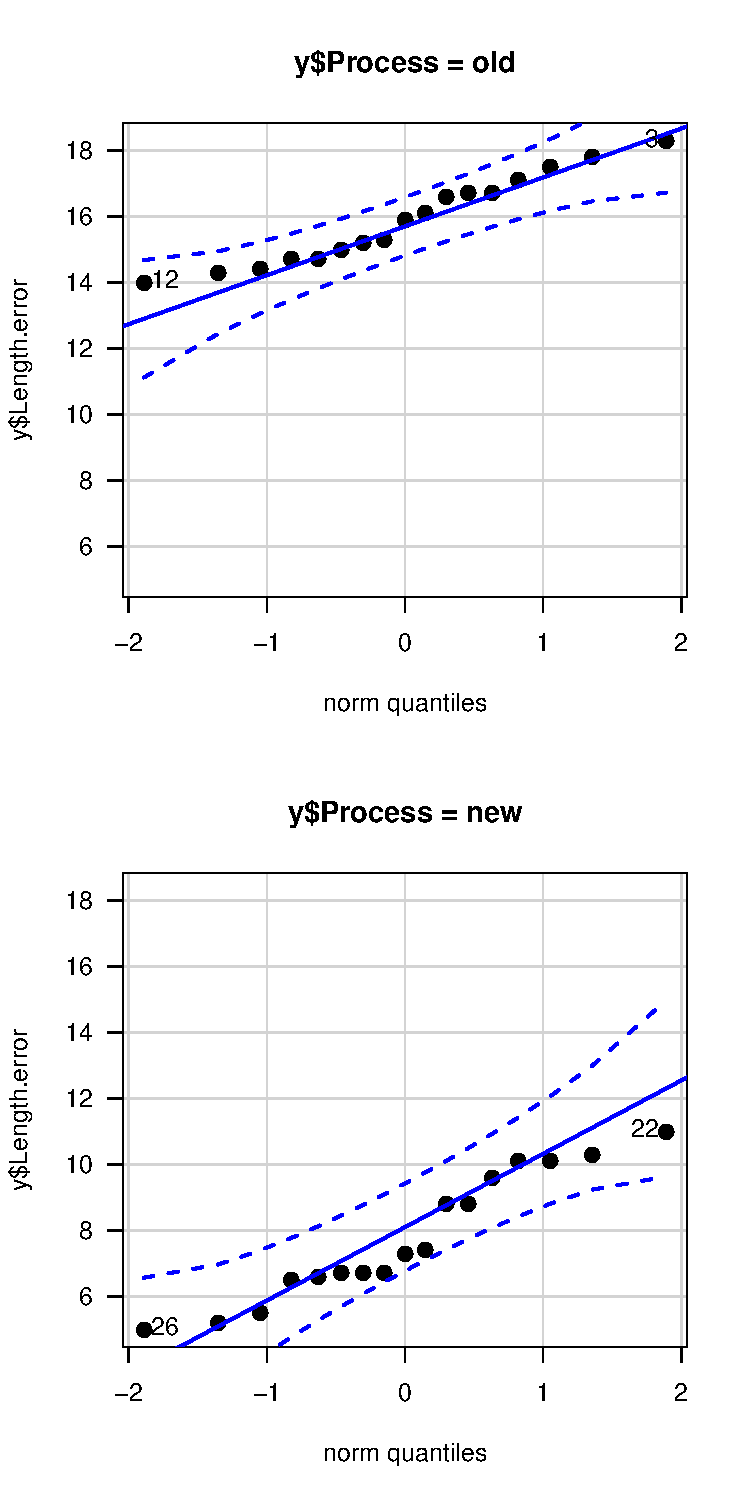
\includegraphics[width=.45\textwidth]{../figs/steelrodsqq.pdf}};
\end{tikzpicture}
\end{ftstf}

%=====

\begin{ftstf}
{Comparison of two means}
{Example: Length of steel rods}
The assumptions of the test must be verified. In this particular case:

\bitems Normality of the residuals;
\item \alert{Equality of variance of the residuals};
\item Independence of the residuals.
\eitem
\begin{rcode}
> with(y,
+      fligner.test(Length.error~Process))
Fligner-Killeen test of homogeneity of variances
data:  Length.error by Process
Fligner-Killeen:med chi-squared = 1.6837, 
df = 1, p-value = 0.1944

> plot(x=rep(means[2:1],
+            each=n),
+      y=resid,
+      xlab="mean",
+      pch=16,
+      cex=1.5,
+      las=1)
\end{rcode}
\begin{tikzpicture}[remember picture,overlay]
\node[anchor=south east,yshift=-10pt,xshift=10pt] at (current page.south east) {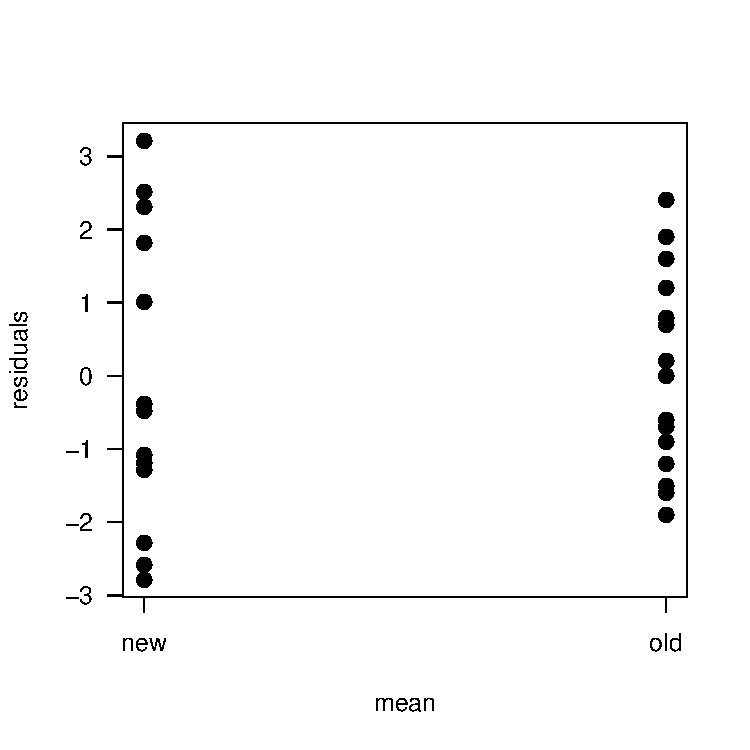
\includegraphics[width=.45\textwidth]{../figs/steelrodsvar.pdf}};
\end{tikzpicture}
\end{ftstf}

%=====

\begin{ftst}
{Comparison of two means}
{Example: Length of steel rods}
The assumptions of the test must be verified. In this particular case:

\bitems Normality of the residuals;
\item Equality of variance of the residuals;
\item \alert{Independence of the residuals}.
\eitem
As mentioned in an earlier lecture, there is no general test for the independence assumption, and it has to be guaranteed in the design phase. 
\vhalf
One can at most test for serial autocorrelation in the residuals using Durbin-Watson's test, but this test is absolutely dependent on the ordering of the observations - very useful to detect ordering-related trends in the residuals, but not much more than that.
\end{ftst}

%=====

%\begin{ftstf}
%{Comparison of two means}
%{Example: Length of steel rods}
%The assumptions of the test must be verified. In this particular case:
%
%\bitems Normality of the residuals;
%\item Equality of variance of the residuals;
%\item \alert{Independence of the residuals}.
%\eitem
%\begin{rcode}
%> library(lmtest)
%> with(y,
%+      dwtest(Length.error~Process))
%Durbin-Watson test
%data:  Length.error ~ Process
%DW = 2.2215, p-value = 0.6838
%alternative hypothesis: true autocorrelation 
%is greater than 0
%
%> plot(resid,
%+      pch=16,
%+      cex=1.5,
%+      type="b",
%+      las=1)
%\end{rcode}
%\begin{tikzpicture}[remember picture,overlay]
%\node[anchor=south east,yshift=-10pt,xshift=10pt] at (current page.south east) {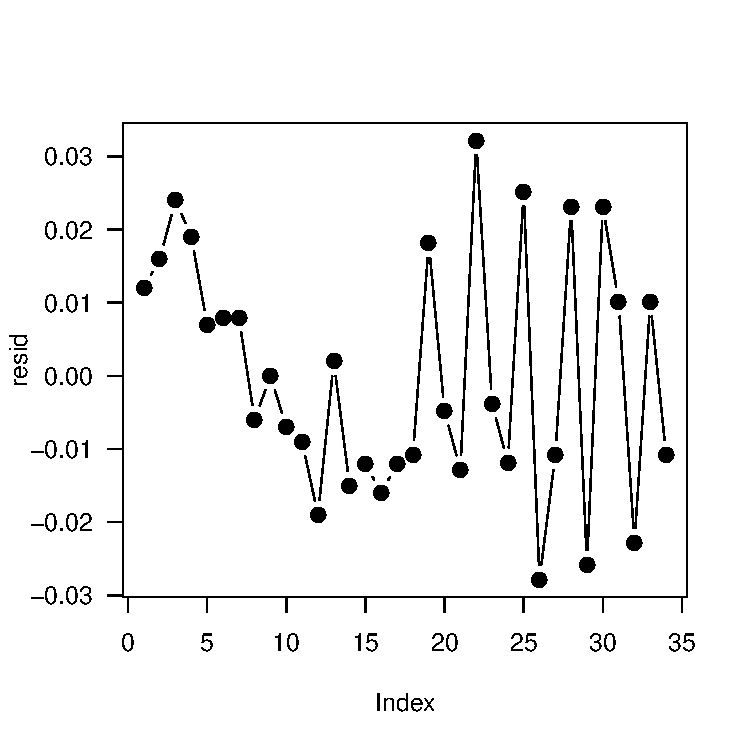
\includegraphics[width=.45\textwidth]{../figs/steelrodsind.pdf}};
%\end{tikzpicture}
%\end{ftstf}

%=====

\begin{ftst}
{Comparison of two means}
{Unequal variances}
Suppose now a more general case, in which the variances of the two populations are unknown and cannot be assumed equal.
\vone 
For this cases, a modification on the t-test called \textit{Welch's t test} is usually employed. The Welch statistic can be calculated as:
\beqs t^*_0 = \frac{\bar{y_1} - \bar{y_2}}{\sqrt{\frac{s_1^2}{n_1} + \frac{s_2^2}{n_2}}}\eqs
\vhalf
Under the null hypothesis $t^*_0$  is distributed approximately as a $t_{\nu}$ distribution, with:
\beqs  \nu = \frac{\left(\frac{s_1^2}{n_1} + \frac{s_2^2}{n_2}\right)^2}{\frac{\left(s_1^2/n_1\right)^2}{n_1-1} + \frac{\left(s_2^2/n_2\right)^2}{n_2-1}}\eqs
\end{ftst}

%=====

\begin{ftstf}
{Comparison of two means}
{Unequal variances}
To illustrate the use of this technique, we can use the same data from the previous example\footnote[2]{Notice that this would not be necessary, since the data collected in the previous example did not violate the equality of variances assumption.}:
\vhalf
\begin{Verbatim}[fontsize=\scriptsize]
> with(y,
+      t.test(Length.error~Process,
+             alternative = "two.sided",
+             mu = 0,
+             var.equal = FALSE,
+             conf.level = 0.95))
Welch Two Sample t-test
data:  Length.error by Process
t = -14.312, df = 28.386, p-value = 1.645e-14
alternative hypothesis: true difference in means is not equal to 0
95 percent confidence interval:
 -0.09278780 -0.06956515
sample estimates:
mean in group new mean in group old 
       0.07782353        0.15900000 
\end{Verbatim}
\vone
\end{ftstf}







%=====


\begin{ftst}
{Bibliography}
{\ }
\scriptsize
\textbf{Required reading}

\benums D.C. Montgomery, G.C. Runger, \textit{Applied Statistics and Probability for Engineers}, Ch. 10. 5th ed., Wiley, 2010.; \textbf{OR}
\item D.C. Montgomery, \textit{Design and Analysis of Experiments}, Ch. 2. 5th ed., Wiley, 2005;
\item R. Nuzzo, \textit{Scientific method: Statistical errors}, Nature 506(7487) - \url{http://goo.gl/Kbq6Rc}
\eenum

\textbf{Recommended reading}

\benums P. Mathews, \textit{Sample Size Calculations: Practical Methods for Engineers and Scientists}, Ch. 1-2, 1st ed., MMB, 2010.
\item Radiolab (podcast): \url{http://radiolab.org}
\eenum
\end{ftst}

%=====

\begin{ftstf}{About this material}{Conditions of use and referencing}
\centering\footnotesize This work is licensed under the Creative Commons CC BY-NC-SA 4.0 license\\(Attribution Non-Commercial Share Alike International License version 4.0).\\
\vhalf
\url{http://creativecommons.org/licenses/by-nc-sa/4.0/}\\
\vone
\footnotesize Please reference this work as:\\
\footnotesize \flushleft Felipe Campelo (2015), \textit{Lecture Notes on Design and Analysis of Experiments}.\\Online: {\scriptsize\url{https://github.com/fcampelo/Design-and-Analysis-of-Experiments}}\\
Version 2.11, Chapter 6; Creative Commons BY-NC-SA 4.0.\\

\begin{Verbatim}[fontsize=\tiny]
    @Misc{Campelo2015-01,
      title={Lecture Notes on Design and Analysis of Experiments},
      author={Felipe Campelo},
      howPublished={\url{https://github.com/fcampelo/Design-and-Analysis-of-Experiments}},
      year={2015},
      note={Version 2.11, Chapter 6; Creative Commons BY-NC-SA 4.0.},
    }
\end{Verbatim}

\begin{tikzpicture} [remember picture,overlay]
\node[anchor=south,yshift=0pt] at (current page.south){ \includegraphics[width=.2\textwidth]{../figs/CCSomerights.png}};
\end{tikzpicture}
\end{ftstf}


\end{document}